\documentclass[1p]{elsarticle_modified}
%\bibliographystyle{elsarticle-num}

%\usepackage[colorlinks]{hyperref}
%\usepackage{abbrmath_seonhwa} %\Abb, \Ascr, \Acal ,\Abf, \Afrak
\usepackage{amsfonts}
\usepackage{amssymb}
\usepackage{amsmath}
\usepackage{amsthm}
\usepackage{scalefnt}
\usepackage{amsbsy}
\usepackage{kotex}
\usepackage{caption}
\usepackage{subfig}
\usepackage{color}
\usepackage{graphicx}
\usepackage{xcolor} %% white, black, red, green, blue, cyan, magenta, yellow
\usepackage{float}
\usepackage{setspace}
\usepackage{hyperref}

\usepackage{tikz}
\usetikzlibrary{arrows}

\usepackage{multirow}
\usepackage{array} % fixed length table
\usepackage{hhline}

%%%%%%%%%%%%%%%%%%%%%
\makeatletter
\renewcommand*\env@matrix[1][\arraystretch]{%
	\edef\arraystretch{#1}%
	\hskip -\arraycolsep
	\let\@ifnextchar\new@ifnextchar
	\array{*\c@MaxMatrixCols c}}
\makeatother %https://tex.stackexchange.com/questions/14071/how-can-i-increase-the-line-spacing-in-a-matrix
%%%%%%%%%%%%%%%

\usepackage[normalem]{ulem}

\newcommand{\msout}[1]{\ifmmode\text{\sout{\ensuremath{#1}}}\else\sout{#1}\fi}
%SOURCE: \msout is \stkout macro in https://tex.stackexchange.com/questions/20609/strikeout-in-math-mode

\newcommand{\cancel}[1]{
	\ifmmode
	{\color{red}\msout{#1}}
	\else
	{\color{red}\sout{#1}}
	\fi
}

\newcommand{\add}[1]{
	{\color{blue}\uwave{#1}}
}

\newcommand{\replace}[2]{
	\ifmmode
	{\color{red}\msout{#1}}{\color{blue}\uwave{#2}}
	\else
	{\color{red}\sout{#1}}{\color{blue}\uwave{#2}}
	\fi
}

\newcommand{\Sol}{\mathcal{S}} %segment
\newcommand{\D}{D} %diagram
\newcommand{\A}{\mathcal{A}} %arc


%%%%%%%%%%%%%%%%%%%%%%%%%%%%%5 test

\def\sl{\operatorname{\textup{SL}}(2,\Cbb)}
\def\psl{\operatorname{\textup{PSL}}(2,\Cbb)}
\def\quan{\mkern 1mu \triangleright \mkern 1mu}

\theoremstyle{definition}
\newtheorem{thm}{Theorem}[section]
\newtheorem{prop}[thm]{Proposition}
\newtheorem{lem}[thm]{Lemma}
\newtheorem{ques}[thm]{Question}
\newtheorem{cor}[thm]{Corollary}
\newtheorem{defn}[thm]{Definition}
\newtheorem{exam}[thm]{Example}
\newtheorem{rmk}[thm]{Remark}
\newtheorem{alg}[thm]{Algorithm}

\newcommand{\I}{\sqrt{-1}}
\begin{document}

%\begin{frontmatter}
%
%\title{Boundary parabolic representations of knots up to 8 crossings}
%
%%% Group authors per affiliation:
%\author{Yunhi Cho} 
%\address{Department of Mathematics, University of Seoul, Seoul, Korea}
%\ead{yhcho@uos.ac.kr}
%
%
%\author{Seonhwa Kim} %\fnref{s_kim}}
%\address{Center for Geometry and Physics, Institute for Basic Science, Pohang, 37673, Korea}
%\ead{ryeona17@ibs.re.kr}
%
%\author{Hyuk Kim}
%\address{Department of Mathematical Sciences, Seoul National University, Seoul 08826, Korea}
%\ead{hyukkim@snu.ac.kr}
%
%\author{Seokbeom Yoon}
%\address{Department of Mathematical Sciences, Seoul National University, Seoul, 08826,  Korea}
%\ead{sbyoon15@snu.ac.kr}
%
%\begin{abstract}
%We find all boundary parabolic representation of knots up to 8 crossings.
%
%\end{abstract}
%\begin{keyword}
%    \MSC[2010] 57M25 
%\end{keyword}
%
%\end{frontmatter}

%\linenumbers
%\tableofcontents
%
\newcommand\colored[1]{\textcolor{white}{\rule[-0.35ex]{0.8em}{1.4ex}}\kern-0.8em\color{red} #1}%
%\newcommand\colored[1]{\textcolor{white}{ #1}\kern-2.17ex	\textcolor{white}{ #1}\kern-1.81ex	\textcolor{white}{ #1}\kern-2.15ex\color{red}#1	}

{\Large $\underline{12n_{0015}~(K12n_{0015})}$}

\setlength{\tabcolsep}{10pt}
\renewcommand{\arraystretch}{1.6}
\vspace{1cm}\begin{tabular}{m{100pt}>{\centering\arraybackslash}m{274pt}}
\multirow{5}{120pt}{
	\centering
	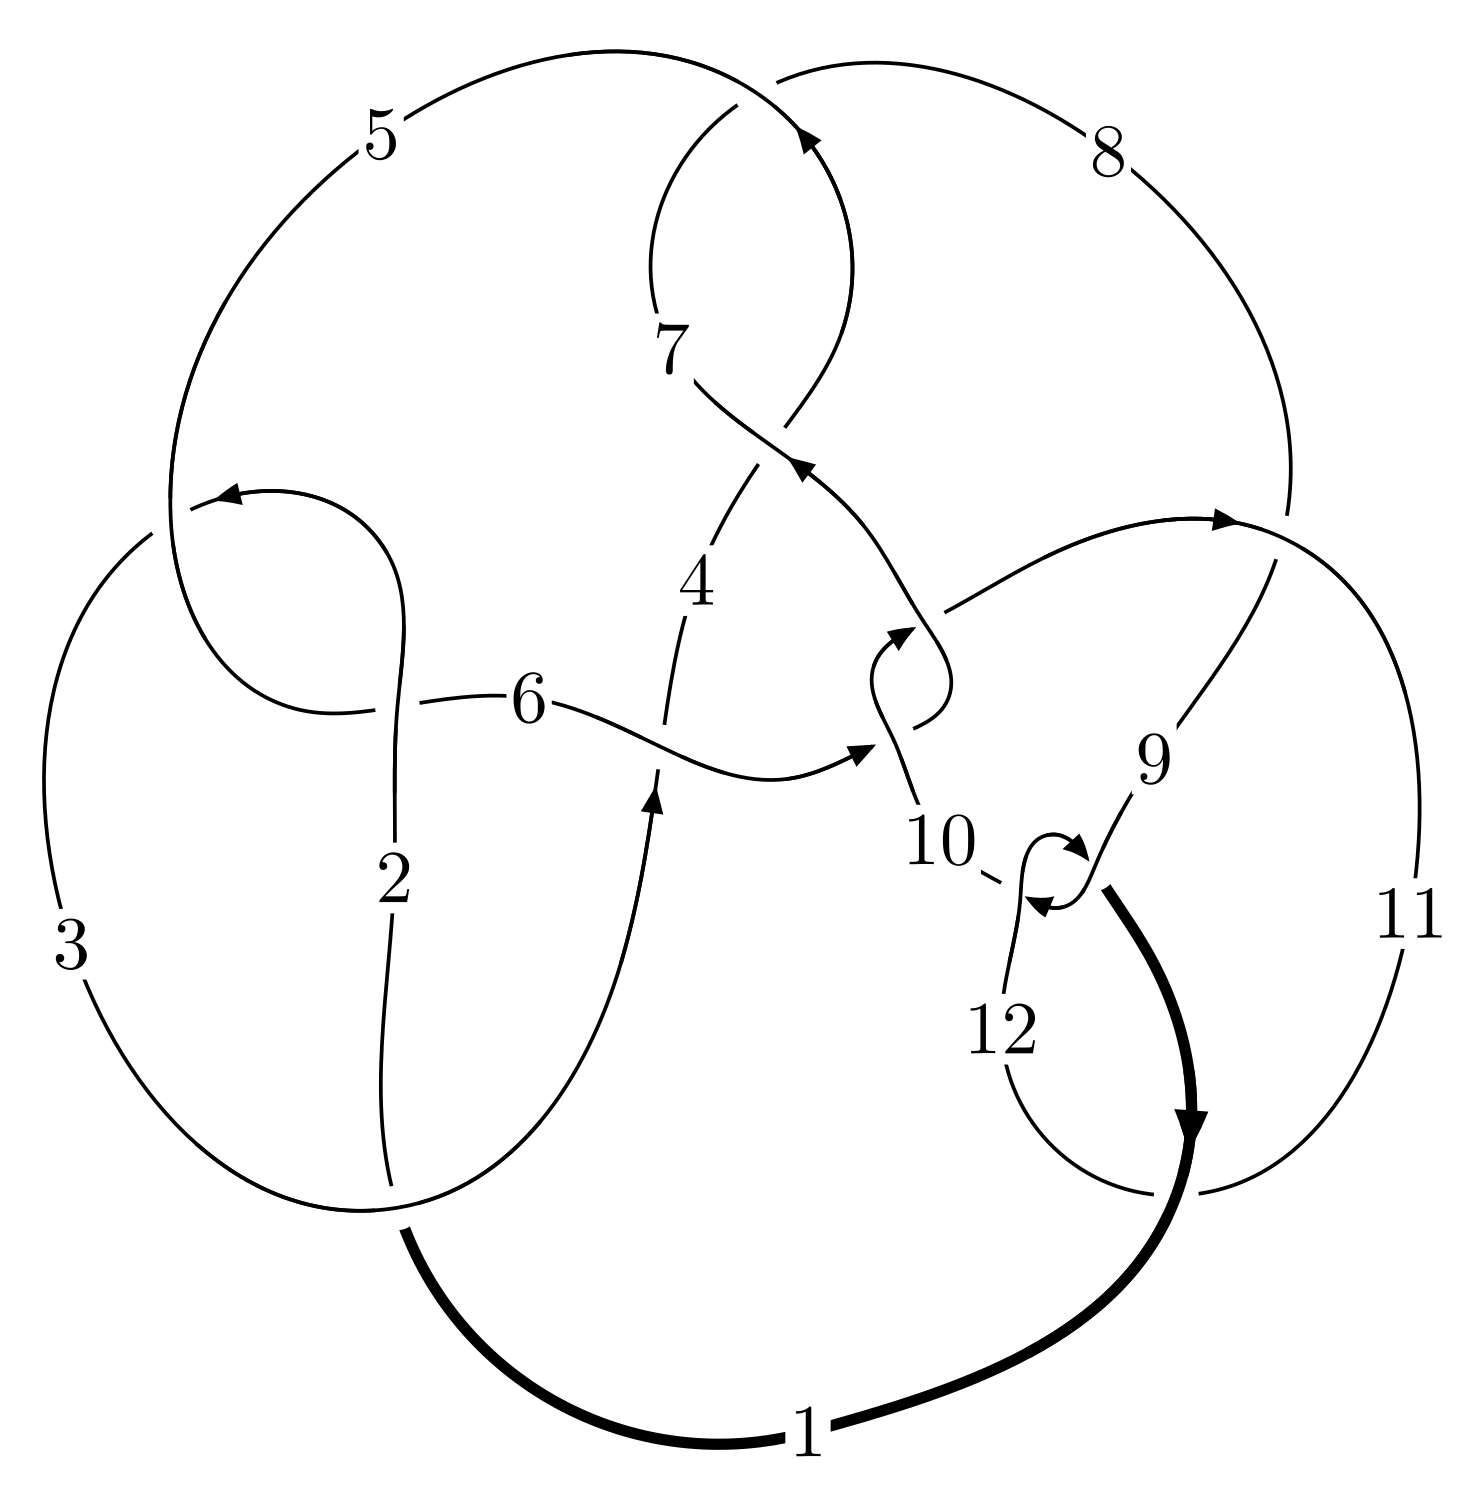
\includegraphics[width=112pt]{../../../GIT/diagram.site/Diagrams/png/2104_12n_0015.png}\\
\ \ \ A knot diagram\footnotemark}&
\allowdisplaybreaks
\textbf{Linearized knot diagam} \\
\cline{2-2}
 &
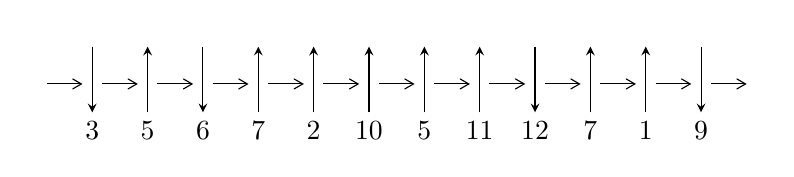
\begin{tikzpicture}[x=20pt, y=17pt]
	% nodes
	\node (C0) at (0, 0) {};
	\node (C1) at (1, 0) {};
	\node (C1U) at (1, +1) {};
	\node (C1D) at (1, -1) {3};

	\node (C2) at (2, 0) {};
	\node (C2U) at (2, +1) {};
	\node (C2D) at (2, -1) {5};

	\node (C3) at (3, 0) {};
	\node (C3U) at (3, +1) {};
	\node (C3D) at (3, -1) {6};

	\node (C4) at (4, 0) {};
	\node (C4U) at (4, +1) {};
	\node (C4D) at (4, -1) {7};

	\node (C5) at (5, 0) {};
	\node (C5U) at (5, +1) {};
	\node (C5D) at (5, -1) {2};

	\node (C6) at (6, 0) {};
	\node (C6U) at (6, +1) {};
	\node (C6D) at (6, -1) {10};

	\node (C7) at (7, 0) {};
	\node (C7U) at (7, +1) {};
	\node (C7D) at (7, -1) {5};

	\node (C8) at (8, 0) {};
	\node (C8U) at (8, +1) {};
	\node (C8D) at (8, -1) {11};

	\node (C9) at (9, 0) {};
	\node (C9U) at (9, +1) {};
	\node (C9D) at (9, -1) {12};

	\node (C10) at (10, 0) {};
	\node (C10U) at (10, +1) {};
	\node (C10D) at (10, -1) {7};

	\node (C11) at (11, 0) {};
	\node (C11U) at (11, +1) {};
	\node (C11D) at (11, -1) {1};

	\node (C12) at (12, 0) {};
	\node (C12U) at (12, +1) {};
	\node (C12D) at (12, -1) {9};
	\node (C13) at (13, 0) {};

	% arrows
	\draw[->,>={angle 60}]
	(C0) edge (C1) (C1) edge (C2) (C2) edge (C3) (C3) edge (C4) (C4) edge (C5) (C5) edge (C6) (C6) edge (C7) (C7) edge (C8) (C8) edge (C9) (C9) edge (C10) (C10) edge (C11) (C11) edge (C12) (C12) edge (C13) ;	\draw[->,>=stealth]
	(C1U) edge (C1D) (C2D) edge (C2U) (C3U) edge (C3D) (C4D) edge (C4U) (C5D) edge (C5U) (C6D) edge (C6U) (C7D) edge (C7U) (C8D) edge (C8U) (C9U) edge (C9D) (C10D) edge (C10U) (C11D) edge (C11U) (C12U) edge (C12D) ;
	\end{tikzpicture} \\
\hhline{~~} \\& 
\textbf{Solving Sequence} \\ \cline{2-2} 
 &
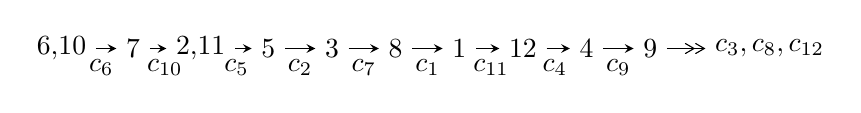
\begin{tikzpicture}[x=23pt, y=7pt]
	% node
	\node (A0) at (-1/8, 0) {6,10};
	\node (A1) at (1, 0) {7};
	\node (A2) at (33/16, 0) {2,11};
	\node (A3) at (25/8, 0) {5};
	\node (A4) at (33/8, 0) {3};
	\node (A5) at (41/8, 0) {8};
	\node (A6) at (49/8, 0) {1};
	\node (A7) at (57/8, 0) {12};
	\node (A8) at (65/8, 0) {4};
	\node (A9) at (73/8, 0) {9};
	\node (C1) at (1/2, -1) {$c_{6}$};
	\node (C2) at (3/2, -1) {$c_{10}$};
	\node (C3) at (21/8, -1) {$c_{5}$};
	\node (C4) at (29/8, -1) {$c_{2}$};
	\node (C5) at (37/8, -1) {$c_{7}$};
	\node (C6) at (45/8, -1) {$c_{1}$};
	\node (C7) at (53/8, -1) {$c_{11}$};
	\node (C8) at (61/8, -1) {$c_{4}$};
	\node (C9) at (69/8, -1) {$c_{9}$};
	\node (A10) at (11, 0) {$c_{3},c_{8},c_{12}$};

	% edge
	\draw[->,>=stealth]	
	(A0) edge (A1) (A1) edge (A2) (A2) edge (A3) (A3) edge (A4) (A4) edge (A5) (A5) edge (A6) (A6) edge (A7) (A7) edge (A8) (A8) edge (A9) ;
	\draw[->>,>={angle 60}]	
	(A9) edge (A10);
\end{tikzpicture} \\ 

\end{tabular} \\

\footnotetext{
The image of knot diagram is generated by the software ``\textbf{Draw programme}" developed by Andrew Bartholomew(\url{http://www.layer8.co.uk/maths/draw/index.htm\#Running-draw}), where we modified some parts for our purpose(\url{https://github.com/CATsTAILs/LinksPainter}).
}\phantom \\ \newline 
\centering \textbf{Ideals for irreducible components\footnotemark of $X_{\text{par}}$} 
 
\begin{align*}
I^u_{1}&=\langle 
1.50022\times10^{125} u^{64}+4.36424\times10^{125} u^{63}+\cdots+3.54215\times10^{125} b-7.96745\times10^{124},\\
\phantom{I^u_{1}}&\phantom{= \langle  }-2.95873\times10^{125} u^{64}-9.80937\times10^{125} u^{63}+\cdots+3.54215\times10^{125} a-9.49669\times10^{125},\;u^{65}+3 u^{64}+\cdots- u^2+1\rangle \\
I^u_{2}&=\langle 
u^3 a- u^2 a+u^3- a u- u^2+b- a- u-1,\;u^4 a-2 u^3 a-4 u^4- u^2 a+5 u^3+a^2+3 a u+8 u^2+a-8 u-3,\\
\phantom{I^u_{2}}&\phantom{= \langle  }u^5- u^4-2 u^3+u^2+u+1\rangle \\
\\
\end{align*}
\raggedright * 2 irreducible components of $\dim_{\mathbb{C}}=0$, with total 75 representations.\\
\footnotetext{All coefficients of polynomials are rational numbers. But the coefficients are sometimes approximated in decimal forms when there is not enough margin.}
\newpage
\renewcommand{\arraystretch}{1}
\centering \section*{I. $I^u_{1}= \langle 1.50\times10^{125} u^{64}+4.36\times10^{125} u^{63}+\cdots+3.54\times10^{125} b-7.97\times10^{124},\;-2.96\times10^{125} u^{64}-9.81\times10^{125} u^{63}+\cdots+3.54\times10^{125} a-9.50\times10^{125},\;u^{65}+3 u^{64}+\cdots- u^2+1 \rangle$}
\flushleft \textbf{(i) Arc colorings}\\
\begin{tabular}{m{7pt} m{180pt} m{7pt} m{180pt} }
\flushright $a_{6}=$&$\begin{pmatrix}1\\0\end{pmatrix}$ \\
\flushright $a_{10}=$&$\begin{pmatrix}0\\u\end{pmatrix}$ \\
\flushright $a_{7}=$&$\begin{pmatrix}1\\- u^2\end{pmatrix}$ \\
\flushright $a_{2}=$&$\begin{pmatrix}0.835293 u^{64}+2.76933 u^{63}+\cdots+1.71444 u+2.68105\\-0.423534 u^{64}-1.23209 u^{63}+\cdots+1.25883 u+0.224932\end{pmatrix}$ \\
\flushright $a_{11}=$&$\begin{pmatrix}u\\- u^3+u\end{pmatrix}$ \\
\flushright $a_{5}=$&$\begin{pmatrix}0.345381 u^{64}+0.473837 u^{63}+\cdots-1.23941 u+2.97738\\-0.310281 u^{64}-0.952665 u^{63}+\cdots+1.07920 u-0.578999\end{pmatrix}$ \\
\flushright $a_{3}=$&$\begin{pmatrix}0.154488 u^{64}-0.107654 u^{63}+\cdots-1.02424 u+2.50407\\-0.0606760 u^{64}-0.279839 u^{63}+\cdots+0.948980 u-0.490002\end{pmatrix}$ \\
\flushright $a_{8}=$&$\begin{pmatrix}0.206883 u^{64}+0.609928 u^{63}+\cdots-1.00346 u-0.732547\\-0.383905 u^{64}-1.05169 u^{63}+\cdots+1.00690 u-0.344765\end{pmatrix}$ \\
\flushright $a_{1}=$&$\begin{pmatrix}0.767182 u^{64}+2.19356 u^{63}+\cdots-1.80348 u-0.398504\\0.560299 u^{64}+1.58363 u^{63}+\cdots-0.800020 u+0.334043\end{pmatrix}$ \\
\flushright $a_{12}=$&$\begin{pmatrix}0.376922 u^{64}+0.519176 u^{63}+\cdots+2.21285 u+0.877994\\0.402208 u^{64}+0.524302 u^{63}+\cdots+1.79239 u-0.116295\end{pmatrix}$ \\
\flushright $a_{4}=$&$\begin{pmatrix}0.215164 u^{64}+0.172185 u^{63}+\cdots-1.97322 u+2.99408\\-0.0606760 u^{64}-0.279839 u^{63}+\cdots+0.948980 u-0.490002\end{pmatrix}$ \\
\flushright $a_{9}=$&$\begin{pmatrix}0.323109 u^{64}+0.870589 u^{63}+\cdots-0.236280 u-0.840533\\-0.433466 u^{64}-1.19898 u^{63}+\cdots+1.89031 u-0.540767\end{pmatrix}$\\&\end{tabular}
\flushleft \textbf{(ii) Obstruction class $= -1$}\\~\\
\flushleft \textbf{(iii) Cusp Shapes $= -2.36898 u^{64}-8.01720 u^{63}+\cdots-34.4288 u-0.224583$}\\~\\
\newpage\renewcommand{\arraystretch}{1}
\flushleft \textbf{(iv) u-Polynomials at the component}\newline \\
\begin{tabular}{m{50pt}|m{274pt}}
Crossings & \hspace{64pt}u-Polynomials at each crossing \\
\hline $$\begin{aligned}c_{1}\end{aligned}$$&$\begin{aligned}
&u^{65}+36 u^{64}+\cdots-153 u-1
\end{aligned}$\\
\hline $$\begin{aligned}c_{2},c_{5}\end{aligned}$$&$\begin{aligned}
&u^{65}+6 u^{64}+\cdots-5 u-1
\end{aligned}$\\
\hline $$\begin{aligned}c_{3}\end{aligned}$$&$\begin{aligned}
&u^{65}-6 u^{64}+\cdots-3141 u-1282
\end{aligned}$\\
\hline $$\begin{aligned}c_{4},c_{7}\end{aligned}$$&$\begin{aligned}
&u^{65}+5 u^{64}+\cdots-13312 u^2-1024
\end{aligned}$\\
\hline $$\begin{aligned}c_{6},c_{10}\end{aligned}$$&$\begin{aligned}
&u^{65}-3 u^{64}+\cdots+u^2-1
\end{aligned}$\\
\hline $$\begin{aligned}c_{8}\end{aligned}$$&$\begin{aligned}
&u^{65}+3 u^{64}+\cdots+969 u-578
\end{aligned}$\\
\hline $$\begin{aligned}c_{9},c_{12}\end{aligned}$$&$\begin{aligned}
&u^{65}-3 u^{64}+\cdots+8 u-1
\end{aligned}$\\
\hline $$\begin{aligned}c_{11}\end{aligned}$$&$\begin{aligned}
&u^{65}-29 u^{64}+\cdots+2 u+1
\end{aligned}$\\
\hline
\end{tabular}\\~\\
\newpage\renewcommand{\arraystretch}{1}
\flushleft \textbf{(v) Riley Polynomials at the component}\newline \\
\begin{tabular}{m{50pt}|m{274pt}}
Crossings & \hspace{64pt}Riley Polynomials at each crossing \\
\hline $$\begin{aligned}c_{1}\end{aligned}$$&$\begin{aligned}
&y^{65}-8 y^{64}+\cdots+10327 y-1
\end{aligned}$\\
\hline $$\begin{aligned}c_{2},c_{5}\end{aligned}$$&$\begin{aligned}
&y^{65}+36 y^{64}+\cdots-153 y-1
\end{aligned}$\\
\hline $$\begin{aligned}c_{3}\end{aligned}$$&$\begin{aligned}
&y^{65}-52 y^{64}+\cdots-241954815 y-1643524
\end{aligned}$\\
\hline $$\begin{aligned}c_{4},c_{7}\end{aligned}$$&$\begin{aligned}
&y^{65}+55 y^{64}+\cdots-27262976 y-1048576
\end{aligned}$\\
\hline $$\begin{aligned}c_{6},c_{10}\end{aligned}$$&$\begin{aligned}
&y^{65}-15 y^{64}+\cdots+2 y-1
\end{aligned}$\\
\hline $$\begin{aligned}c_{8}\end{aligned}$$&$\begin{aligned}
&y^{65}+5 y^{64}+\cdots-4574003 y-334084
\end{aligned}$\\
\hline $$\begin{aligned}c_{9},c_{12}\end{aligned}$$&$\begin{aligned}
&y^{65}+29 y^{64}+\cdots+2 y-1
\end{aligned}$\\
\hline $$\begin{aligned}c_{11}\end{aligned}$$&$\begin{aligned}
&y^{65}+17 y^{64}+\cdots-142 y-1
\end{aligned}$\\
\hline
\end{tabular}\\~\\
\newpage\flushleft \textbf{(vi) Complex Volumes and Cusp Shapes}
$$\begin{array}{c|c|c}  
\text{Solutions to }I^u_{1}& \I (\text{vol} + \sqrt{-1}CS) & \text{Cusp shape}\\
 \hline 
\begin{aligned}
u &= \phantom{-}0.628102 + 0.569155 I \\
a &= -0.40185 + 1.73582 I \\
b &= \phantom{-}0.448292 + 1.291450 I\end{aligned}
 & -1.16500 + 7.59687 I & \phantom{-}3.63163 - 10.87893 I \\ \hline\begin{aligned}
u &= \phantom{-}0.628102 - 0.569155 I \\
a &= -0.40185 - 1.73582 I \\
b &= \phantom{-}0.448292 - 1.291450 I\end{aligned}
 & -1.16500 - 7.59687 I & \phantom{-}3.63163 + 10.87893 I \\ \hline\begin{aligned}
u &= -0.565212 + 0.623133 I \\
a &= -0.32719 - 1.87544 I \\
b &= \phantom{-}0.344749 - 1.222650 I\end{aligned}
 & -2.37364 - 2.97409 I & \phantom{-}0.03419 + 4.98688 I \\ \hline\begin{aligned}
u &= -0.565212 - 0.623133 I \\
a &= -0.32719 + 1.87544 I \\
b &= \phantom{-}0.344749 + 1.222650 I\end{aligned}
 & -2.37364 + 2.97409 I & \phantom{-}0.03419 - 4.98688 I \\ \hline\begin{aligned}
u &= \phantom{-}0.072366 + 0.781453 I \\
a &= \phantom{-}1.19704 + 1.78785 I \\
b &= \phantom{-}0.152981 + 0.671120 I\end{aligned}
 & \phantom{-}0.24332 - 1.46975 I & \phantom{-}2.96650 + 0.84122 I \\ \hline\begin{aligned}
u &= \phantom{-}0.072366 - 0.781453 I \\
a &= \phantom{-}1.19704 - 1.78785 I \\
b &= \phantom{-}0.152981 - 0.671120 I\end{aligned}
 & \phantom{-}0.24332 + 1.46975 I & \phantom{-}2.96650 - 0.84122 I \\ \hline\begin{aligned}
u &= -0.340961 + 0.698038 I \\
a &= \phantom{-}0.19869 - 2.27298 I \\
b &= \phantom{-}0.233975 - 0.974531 I\end{aligned}
 & -1.64164 - 2.15616 I & -0.38705 + 4.35750 I \\ \hline\begin{aligned}
u &= -0.340961 - 0.698038 I \\
a &= \phantom{-}0.19869 + 2.27298 I \\
b &= \phantom{-}0.233975 + 0.974531 I\end{aligned}
 & -1.64164 + 2.15616 I & -0.38705 - 4.35750 I \\ \hline\begin{aligned}
u &= -0.725228 + 0.278028 I \\
a &= \phantom{-}1.95932 - 0.44335 I \\
b &= \phantom{-}0.208955 + 0.909618 I\end{aligned}
 & -1.41966 - 0.52874 I & \phantom{-}3.13856 + 2.24700 I \\ \hline\begin{aligned}
u &= -0.725228 - 0.278028 I \\
a &= \phantom{-}1.95932 + 0.44335 I \\
b &= \phantom{-}0.208955 - 0.909618 I\end{aligned}
 & -1.41966 + 0.52874 I & \phantom{-}3.13856 - 2.24700 I\\
 \hline 
 \end{array}$$\newpage$$\begin{array}{c|c|c}  
\text{Solutions to }I^u_{1}& \I (\text{vol} + \sqrt{-1}CS) & \text{Cusp shape}\\
 \hline 
\begin{aligned}
u &= -0.765214 + 0.985370 I \\
a &= -0.15270 - 1.41131 I \\
b &= -0.264359 - 1.359580 I\end{aligned}
 & -7.96046 - 6.18775 I & \phantom{-0.000000 } 0 \\ \hline\begin{aligned}
u &= -0.765214 - 0.985370 I \\
a &= -0.15270 + 1.41131 I \\
b &= -0.264359 + 1.359580 I\end{aligned}
 & -7.96046 + 6.18775 I & \phantom{-0.000000 } 0 \\ \hline\begin{aligned}
u &= -0.855805 + 0.909432 I \\
a &= \phantom{-}0.197635 + 0.609389 I \\
b &= -0.821764 + 0.080284 I\end{aligned}
 & -2.89879 + 3.80873 I & \phantom{-0.000000 } 0 \\ \hline\begin{aligned}
u &= -0.855805 - 0.909432 I \\
a &= \phantom{-}0.197635 - 0.609389 I \\
b &= -0.821764 - 0.080284 I\end{aligned}
 & -2.89879 - 3.80873 I & \phantom{-0.000000 } 0 \\ \hline\begin{aligned}
u &= \phantom{-}0.897889 + 0.886104 I \\
a &= \phantom{-}0.138267 - 0.519755 I \\
b &= -0.856989 + 0.018873 I\end{aligned}
 & -4.61158 + 1.57498 I & \phantom{-0.000000 } 0 \\ \hline\begin{aligned}
u &= \phantom{-}0.897889 - 0.886104 I \\
a &= \phantom{-}0.138267 + 0.519755 I \\
b &= -0.856989 - 0.018873 I\end{aligned}
 & -4.61158 - 1.57498 I & \phantom{-0.000000 } 0 \\ \hline\begin{aligned}
u &= -0.977996 + 0.800120 I \\
a &= \phantom{-}0.160447 + 0.259314 I \\
b &= -0.781893 - 0.251942 I\end{aligned}
 & \phantom{-}1.27467 - 2.98710 I & \phantom{-0.000000 } 0 \\ \hline\begin{aligned}
u &= -0.977996 - 0.800120 I \\
a &= \phantom{-}0.160447 - 0.259314 I \\
b &= -0.781893 + 0.251942 I\end{aligned}
 & \phantom{-}1.27467 + 2.98710 I & \phantom{-0.000000 } 0 \\ \hline\begin{aligned}
u &= \phantom{-}0.734905 + 0.039492 I \\
a &= \phantom{-}0.217205 - 0.011467 I \\
b &= \phantom{-}0.883998 + 0.223037 I\end{aligned}
 & \phantom{-}3.33660 + 2.97737 I & \phantom{-}14.6570 - 4.9725 I \\ \hline\begin{aligned}
u &= \phantom{-}0.734905 - 0.039492 I \\
a &= \phantom{-}0.217205 + 0.011467 I \\
b &= \phantom{-}0.883998 - 0.223037 I\end{aligned}
 & \phantom{-}3.33660 - 2.97737 I & \phantom{-}14.6570 + 4.9725 I\\
 \hline 
 \end{array}$$\newpage$$\begin{array}{c|c|c}  
\text{Solutions to }I^u_{1}& \I (\text{vol} + \sqrt{-1}CS) & \text{Cusp shape}\\
 \hline 
\begin{aligned}
u &= -0.677662 + 0.256690 I \\
a &= -0.554218 - 0.670994 I \\
b &= \phantom{-}0.850990 - 0.944246 I\end{aligned}
 & \phantom{-}2.13495 - 5.98222 I & \phantom{-}10.3042 + 10.3831 I \\ \hline\begin{aligned}
u &= -0.677662 - 0.256690 I \\
a &= -0.554218 + 0.670994 I \\
b &= \phantom{-}0.850990 + 0.944246 I\end{aligned}
 & \phantom{-}2.13495 + 5.98222 I & \phantom{-}10.3042 - 10.3831 I \\ \hline\begin{aligned}
u &= -0.697071 + 0.134831 I \\
a &= -0.208690 - 0.093719 I \\
b &= \phantom{-}0.865604 - 0.650193 I\end{aligned}
 & \phantom{-}2.94313 - 0.27251 I & \phantom{-}13.63116 + 1.74028 I \\ \hline\begin{aligned}
u &= -0.697071 - 0.134831 I \\
a &= -0.208690 + 0.093719 I \\
b &= \phantom{-}0.865604 + 0.650193 I\end{aligned}
 & \phantom{-}2.94313 + 0.27251 I & \phantom{-}13.63116 - 1.74028 I \\ \hline\begin{aligned}
u &= \phantom{-}0.783819 + 1.026080 I \\
a &= -0.143080 + 1.349990 I \\
b &= -0.323635 + 1.327820 I\end{aligned}
 & -9.37380 + 0.62790 I & \phantom{-0.000000 } 0 \\ \hline\begin{aligned}
u &= \phantom{-}0.783819 - 1.026080 I \\
a &= -0.143080 - 1.349990 I \\
b &= -0.323635 - 1.327820 I\end{aligned}
 & -9.37380 - 0.62790 I & \phantom{-0.000000 } 0 \\ \hline\begin{aligned}
u &= \phantom{-}0.583045 + 0.371142 I \\
a &= -0.94998 + 1.34055 I \\
b &= \phantom{-}0.642745 + 1.066730 I\end{aligned}
 & \phantom{-}0.97209 + 2.48020 I & \phantom{-}8.17214 - 4.93777 I \\ \hline\begin{aligned}
u &= \phantom{-}0.583045 - 0.371142 I \\
a &= -0.94998 - 1.34055 I \\
b &= \phantom{-}0.642745 - 1.066730 I\end{aligned}
 & \phantom{-}0.97209 - 2.48020 I & \phantom{-}8.17214 + 4.93777 I \\ \hline\begin{aligned}
u &= \phantom{-}0.980745 + 0.879226 I \\
a &= -0.009190 - 0.355180 I \\
b &= -0.952450 + 0.203308 I\end{aligned}
 & -4.36918 + 4.99205 I & \phantom{-0.000000 } 0 \\ \hline\begin{aligned}
u &= \phantom{-}0.980745 - 0.879226 I \\
a &= -0.009190 + 0.355180 I \\
b &= -0.952450 - 0.203308 I\end{aligned}
 & -4.36918 - 4.99205 I & \phantom{-0.000000 } 0\\
 \hline 
 \end{array}$$\newpage$$\begin{array}{c|c|c}  
\text{Solutions to }I^u_{1}& \I (\text{vol} + \sqrt{-1}CS) & \text{Cusp shape}\\
 \hline 
\begin{aligned}
u &= -0.674850\phantom{ +0.000000I} \\
a &= \phantom{-}0.446292\phantom{ +0.000000I} \\
b &= \phantom{-}0.463057\phantom{ +0.000000I}\end{aligned}
 & \phantom{-}1.16666\phantom{ +0.000000I} & \phantom{-}8.48480\phantom{ +0.000000I} \\ \hline\begin{aligned}
u &= -1.326940 + 0.154775 I \\
a &= \phantom{-}0.982376 + 0.410900 I \\
b &= -0.273052 + 0.826180 I\end{aligned}
 & \phantom{-}1.92758 - 1.33174 I & \phantom{-0.000000 } 0 \\ \hline\begin{aligned}
u &= -1.326940 - 0.154775 I \\
a &= \phantom{-}0.982376 - 0.410900 I \\
b &= -0.273052 - 0.826180 I\end{aligned}
 & \phantom{-}1.92758 + 1.33174 I & \phantom{-0.000000 } 0 \\ \hline\begin{aligned}
u &= \phantom{-}0.580701 + 0.321504 I \\
a &= \phantom{-}2.76581 + 0.85928 I \\
b &= \phantom{-}0.345091 - 0.954683 I\end{aligned}
 & -0.87681 - 4.22656 I & \phantom{-}6.95306 + 2.39808 I \\ \hline\begin{aligned}
u &= \phantom{-}0.580701 - 0.321504 I \\
a &= \phantom{-}2.76581 - 0.85928 I \\
b &= \phantom{-}0.345091 + 0.954683 I\end{aligned}
 & -0.87681 + 4.22656 I & \phantom{-}6.95306 - 2.39808 I \\ \hline\begin{aligned}
u &= -1.003250 + 0.884542 I \\
a &= -0.060369 + 0.304416 I \\
b &= -0.985091 - 0.260120 I\end{aligned}
 & -2.47713 - 10.45070 I & \phantom{-0.000000 } 0 \\ \hline\begin{aligned}
u &= -1.003250 - 0.884542 I \\
a &= -0.060369 - 0.304416 I \\
b &= -0.985091 + 0.260120 I\end{aligned}
 & -2.47713 + 10.45070 I & \phantom{-0.000000 } 0 \\ \hline\begin{aligned}
u &= -0.745935 + 1.160500 I \\
a &= \phantom{-}0.000884 - 1.252980 I \\
b &= -0.361004 - 1.170190 I\end{aligned}
 & -2.81669 + 0.45437 I & \phantom{-0.000000 } 0 \\ \hline\begin{aligned}
u &= -0.745935 - 1.160500 I \\
a &= \phantom{-}0.000884 + 1.252980 I \\
b &= -0.361004 + 1.170190 I\end{aligned}
 & -2.81669 - 0.45437 I & \phantom{-0.000000 } 0 \\ \hline\begin{aligned}
u &= -1.127810 + 0.820945 I \\
a &= \phantom{-}1.24601 + 1.23918 I \\
b &= -0.420609 + 1.227310 I\end{aligned}
 & -6.79571 - 0.50966 I & \phantom{-0.000000 } 0\\
 \hline 
 \end{array}$$\newpage$$\begin{array}{c|c|c}  
\text{Solutions to }I^u_{1}& \I (\text{vol} + \sqrt{-1}CS) & \text{Cusp shape}\\
 \hline 
\begin{aligned}
u &= -1.127810 - 0.820945 I \\
a &= \phantom{-}1.24601 - 1.23918 I \\
b &= -0.420609 - 1.227310 I\end{aligned}
 & -6.79571 + 0.50966 I & \phantom{-0.000000 } 0 \\ \hline\begin{aligned}
u &= \phantom{-}0.849131 + 1.120280 I \\
a &= -0.118188 + 1.192840 I \\
b &= -0.451043 + 1.242660 I\end{aligned}
 & -8.41853 - 3.05895 I & \phantom{-0.000000 } 0 \\ \hline\begin{aligned}
u &= \phantom{-}0.849131 - 1.120280 I \\
a &= -0.118188 - 1.192840 I \\
b &= -0.451043 - 1.242660 I\end{aligned}
 & -8.41853 + 3.05895 I & \phantom{-0.000000 } 0 \\ \hline\begin{aligned}
u &= -0.195377 + 0.553421 I \\
a &= \phantom{-}1.205400 + 0.389629 I \\
b &= -0.0029121 + 0.1179000 I\end{aligned}
 & \phantom{-}0.36359 - 1.66193 I & \phantom{-}2.56838 + 3.46511 I \\ \hline\begin{aligned}
u &= -0.195377 - 0.553421 I \\
a &= \phantom{-}1.205400 - 0.389629 I \\
b &= -0.0029121 - 0.1179000 I\end{aligned}
 & \phantom{-}0.36359 + 1.66193 I & \phantom{-}2.56838 - 3.46511 I \\ \hline\begin{aligned}
u &= \phantom{-}1.12627 + 0.86481 I \\
a &= \phantom{-}1.18250 - 1.30489 I \\
b &= -0.470843 - 1.237780 I\end{aligned}
 & -8.27510 + 6.31962 I & \phantom{-0.000000 } 0 \\ \hline\begin{aligned}
u &= \phantom{-}1.12627 - 0.86481 I \\
a &= \phantom{-}1.18250 + 1.30489 I \\
b &= -0.470843 + 1.237780 I\end{aligned}
 & -8.27510 - 6.31962 I & \phantom{-0.000000 } 0 \\ \hline\begin{aligned}
u &= \phantom{-}0.534053 + 0.202971 I \\
a &= -1.58350 + 0.17037 I \\
b &= \phantom{-}0.633931 + 0.867673 I\end{aligned}
 & \phantom{-}0.62677 + 2.45051 I & \phantom{-}2.30160 - 3.49944 I \\ \hline\begin{aligned}
u &= \phantom{-}0.534053 - 0.202971 I \\
a &= -1.58350 - 0.17037 I \\
b &= \phantom{-}0.633931 - 0.867673 I\end{aligned}
 & \phantom{-}0.62677 - 2.45051 I & \phantom{-}2.30160 + 3.49944 I \\ \hline\begin{aligned}
u &= -0.88456 + 1.14555 I \\
a &= -0.116208 - 1.133810 I \\
b &= -0.494977 - 1.215640 I\end{aligned}
 & -6.25912 + 8.60016 I & \phantom{-0.000000 } 0\\
 \hline 
 \end{array}$$\newpage$$\begin{array}{c|c|c}  
\text{Solutions to }I^u_{1}& \I (\text{vol} + \sqrt{-1}CS) & \text{Cusp shape}\\
 \hline 
\begin{aligned}
u &= -0.88456 - 1.14555 I \\
a &= -0.116208 + 1.133810 I \\
b &= -0.494977 + 1.215640 I\end{aligned}
 & -6.25912 - 8.60016 I & \phantom{-0.000000 } 0 \\ \hline\begin{aligned}
u &= \phantom{-}1.45538 + 0.10222 I \\
a &= \phantom{-}0.757445 + 0.377705 I \\
b &= -0.361366 + 0.750604 I\end{aligned}
 & \phantom{-}5.76923 + 2.96244 I & \phantom{-0.000000 } 0 \\ \hline\begin{aligned}
u &= \phantom{-}1.45538 - 0.10222 I \\
a &= \phantom{-}0.757445 - 0.377705 I \\
b &= -0.361366 - 0.750604 I\end{aligned}
 & \phantom{-}5.76923 - 2.96244 I & \phantom{-0.000000 } 0 \\ \hline\begin{aligned}
u &= \phantom{-}1.11941 + 0.94502 I \\
a &= \phantom{-}1.03658 - 1.40534 I \\
b &= -0.576768 - 1.237090 I\end{aligned}
 & -7.52216 + 10.51980 I & \phantom{-0.000000 } 0 \\ \hline\begin{aligned}
u &= \phantom{-}1.11941 - 0.94502 I \\
a &= \phantom{-}1.03658 + 1.40534 I \\
b &= -0.576768 + 1.237090 I\end{aligned}
 & -7.52216 - 10.51980 I & \phantom{-0.000000 } 0 \\ \hline\begin{aligned}
u &= -1.11499 + 0.96636 I \\
a &= \phantom{-}0.99158 + 1.42922 I \\
b &= -0.608733 + 1.232920 I\end{aligned}
 & -5.4631 - 16.2041 I & \phantom{-0.000000 } 0 \\ \hline\begin{aligned}
u &= -1.11499 - 0.96636 I \\
a &= \phantom{-}0.99158 - 1.42922 I \\
b &= -0.608733 - 1.232920 I\end{aligned}
 & -5.4631 + 16.2041 I & \phantom{-0.000000 } 0 \\ \hline\begin{aligned}
u &= -1.17549 + 0.93342 I \\
a &= \phantom{-}1.01884 + 1.29137 I \\
b &= -0.543560 + 1.174510 I\end{aligned}
 & -1.47035 - 7.97117 I & \phantom{-0.000000 } 0 \\ \hline\begin{aligned}
u &= -1.17549 - 0.93342 I \\
a &= \phantom{-}1.01884 - 1.29137 I \\
b &= -0.543560 - 1.174510 I\end{aligned}
 & -1.47035 + 7.97117 I & \phantom{-0.000000 } 0 \\ \hline\begin{aligned}
u &= -0.039971 + 0.483137 I \\
a &= \phantom{-}4.26633 + 3.79248 I \\
b &= \phantom{-}0.520875 + 0.799810 I\end{aligned}
 & \phantom{-}0.42197 + 3.98006 I & -11.1996 - 14.1267 I\\
 \hline 
 \end{array}$$\newpage$$\begin{array}{c|c|c}  
\text{Solutions to }I^u_{1}& \I (\text{vol} + \sqrt{-1}CS) & \text{Cusp shape}\\
 \hline 
\begin{aligned}
u &= -0.039971 - 0.483137 I \\
a &= \phantom{-}4.26633 - 3.79248 I \\
b &= \phantom{-}0.520875 - 0.799810 I\end{aligned}
 & \phantom{-}0.42197 - 3.98006 I & -11.1996 + 14.1267 I \\ \hline\begin{aligned}
u &= \phantom{-}1.51110 + 0.30215 I \\
a &= \phantom{-}0.932692 - 0.595477 I \\
b &= -0.344026 - 0.883021 I\end{aligned}
 & \phantom{-}5.37755 + 6.09849 I & \phantom{-0.000000 } 0 \\ \hline\begin{aligned}
u &= \phantom{-}1.51110 - 0.30215 I \\
a &= \phantom{-}0.932692 + 0.595477 I \\
b &= -0.344026 + 0.883021 I\end{aligned}
 & \phantom{-}5.37755 - 6.09849 I & \phantom{-0.000000 } 0 \\ \hline\begin{aligned}
u &= \phantom{-}0.199982 + 0.366065 I \\
a &= \phantom{-}7.44696 - 1.05122 I \\
b &= \phantom{-}0.531360 - 0.882027 I\end{aligned}
 & \phantom{-}0.173552 - 0.278194 I & -17.0776 - 31.8991 I \\ \hline\begin{aligned}
u &= \phantom{-}0.199982 - 0.366065 I \\
a &= \phantom{-}7.44696 + 1.05122 I \\
b &= \phantom{-}0.531360 + 0.882027 I\end{aligned}
 & \phantom{-}0.173552 + 0.278194 I & -17.0776 + 31.8991 I\\
 \hline 
 \end{array}$$\newpage\newpage\renewcommand{\arraystretch}{1}
\centering \section*{II. $I^u_{2}= \langle u^3 a- u^2 a+u^3- a u- u^2+b- a- u-1,\;u^4 a-4 u^4+\cdots+a-3,\;u^5- u^4-2 u^3+u^2+u+1 \rangle$}
\flushleft \textbf{(i) Arc colorings}\\
\begin{tabular}{m{7pt} m{180pt} m{7pt} m{180pt} }
\flushright $a_{6}=$&$\begin{pmatrix}1\\0\end{pmatrix}$ \\
\flushright $a_{10}=$&$\begin{pmatrix}0\\u\end{pmatrix}$ \\
\flushright $a_{7}=$&$\begin{pmatrix}1\\- u^2\end{pmatrix}$ \\
\flushright $a_{2}=$&$\begin{pmatrix}a\\- u^3 a+u^2 a- u^3+a u+u^2+a+u+1\end{pmatrix}$ \\
\flushright $a_{11}=$&$\begin{pmatrix}u\\- u^3+u\end{pmatrix}$ \\
\flushright $a_{5}=$&$\begin{pmatrix}u^3 a+u^4- u^2 a- u^3- a u-2 u^2+2 u\\- u^3 a+u^2 a- u^3+a u+u^2+a+u\end{pmatrix}$ \\
\flushright $a_{3}=$&$\begin{pmatrix}u^4-2 u^3- u^2+a+3 u\\- u^3 a+u^2 a- u^3+a u+u^2+a+u\end{pmatrix}$ \\
\flushright $a_{8}=$&$\begin{pmatrix}1\\- u^2\end{pmatrix}$ \\
\flushright $a_{1}=$&$\begin{pmatrix}-1\\0\end{pmatrix}$ \\
\flushright $a_{12}=$&$\begin{pmatrix}- u^3+2 u\\- u^3+u\end{pmatrix}$ \\
\flushright $a_{4}=$&$\begin{pmatrix}u^3 a+u^4- u^2 a- u^3- a u-2 u^2+2 u\\- u^3 a+u^2 a- u^3+a u+u^2+a+u\end{pmatrix}$ \\
\flushright $a_{9}=$&$\begin{pmatrix}- u^2+1\\u^4-2 u^2\end{pmatrix}$\\&\end{tabular}
\flushleft \textbf{(ii) Obstruction class $= 1$}\\~\\
\flushleft \textbf{(iii) Cusp Shapes $= -2 u^4 a+6 u^3 a- u^4-4 u^2 a+2 u^3-7 a u-4 u^2-5 a+u+5$}\\~\\
\newpage\renewcommand{\arraystretch}{1}
\flushleft \textbf{(iv) u-Polynomials at the component}\newline \\
\begin{tabular}{m{50pt}|m{274pt}}
Crossings & \hspace{64pt}u-Polynomials at each crossing \\
\hline $$\begin{aligned}c_{1},c_{3},c_{5}\end{aligned}$$&$\begin{aligned}
&(u^2- u+1)^5
\end{aligned}$\\
\hline $$\begin{aligned}c_{2}\end{aligned}$$&$\begin{aligned}
&(u^2+u+1)^5
\end{aligned}$\\
\hline $$\begin{aligned}c_{4},c_{7}\end{aligned}$$&$\begin{aligned}
&u^{10}
\end{aligned}$\\
\hline $$\begin{aligned}c_{6},c_{8}\end{aligned}$$&$\begin{aligned}
&(u^5- u^4-2 u^3+u^2+u+1)^2
\end{aligned}$\\
\hline $$\begin{aligned}c_{9}\end{aligned}$$&$\begin{aligned}
&(u^5+u^4+2 u^3+u^2+u+1)^2
\end{aligned}$\\
\hline $$\begin{aligned}c_{10}\end{aligned}$$&$\begin{aligned}
&(u^5+u^4-2 u^3- u^2+u-1)^2
\end{aligned}$\\
\hline $$\begin{aligned}c_{11}\end{aligned}$$&$\begin{aligned}
&(u^5+3 u^4+4 u^3+u^2- u-1)^2
\end{aligned}$\\
\hline $$\begin{aligned}c_{12}\end{aligned}$$&$\begin{aligned}
&(u^5- u^4+2 u^3- u^2+u-1)^2
\end{aligned}$\\
\hline
\end{tabular}\\~\\
\newpage\renewcommand{\arraystretch}{1}
\flushleft \textbf{(v) Riley Polynomials at the component}\newline \\
\begin{tabular}{m{50pt}|m{274pt}}
Crossings & \hspace{64pt}Riley Polynomials at each crossing \\
\hline $$\begin{aligned}c_{1},c_{2},c_{3}\\c_{5}\end{aligned}$$&$\begin{aligned}
&(y^2+y+1)^5
\end{aligned}$\\
\hline $$\begin{aligned}c_{4},c_{7}\end{aligned}$$&$\begin{aligned}
&y^{10}
\end{aligned}$\\
\hline $$\begin{aligned}c_{6},c_{8},c_{10}\end{aligned}$$&$\begin{aligned}
&(y^5-5 y^4+8 y^3-3 y^2- y-1)^2
\end{aligned}$\\
\hline $$\begin{aligned}c_{9},c_{12}\end{aligned}$$&$\begin{aligned}
&(y^5+3 y^4+4 y^3+y^2- y-1)^2
\end{aligned}$\\
\hline $$\begin{aligned}c_{11}\end{aligned}$$&$\begin{aligned}
&(y^5- y^4+8 y^3-3 y^2+3 y-1)^2
\end{aligned}$\\
\hline
\end{tabular}\\~\\
\newpage\flushleft \textbf{(vi) Complex Volumes and Cusp Shapes}
$$\begin{array}{c|c|c}  
\text{Solutions to }I^u_{2}& \I (\text{vol} + \sqrt{-1}CS) & \text{Cusp shape}\\
 \hline 
\begin{aligned}
u &= -1.21774\phantom{ +0.000000I} \\
a &= -0.837181 + 0.282010 I \\
b &= \phantom{-}0.500000 + 0.866025 I\end{aligned}
 & \phantom{-}2.40108 + 2.02988 I & \phantom{-}6.80799 - 4.97460 I \\ \hline\begin{aligned}
u &= -1.21774\phantom{ +0.000000I} \\
a &= -0.837181 - 0.282010 I \\
b &= \phantom{-}0.500000 - 0.866025 I\end{aligned}
 & \phantom{-}2.40108 - 2.02988 I & \phantom{-}6.80799 + 4.97460 I \\ \hline\begin{aligned}
u &= -0.309916 + 0.549911 I \\
a &= \phantom{-}2.00919 + 0.91819 I \\
b &= \phantom{-}0.500000 + 0.866025 I\end{aligned}
 & \phantom{-}0.329100 + 0.499304 I & \phantom{-}7.97351 - 4.21865 I \\ \hline\begin{aligned}
u &= -0.309916 + 0.549911 I \\
a &= -1.70942 - 3.06513 I \\
b &= \phantom{-}0.500000 - 0.866025 I\end{aligned}
 & \phantom{-}0.32910 - 3.56046 I & -1.93681 + 7.63956 I \\ \hline\begin{aligned}
u &= -0.309916 - 0.549911 I \\
a &= \phantom{-}2.00919 - 0.91819 I \\
b &= \phantom{-}0.500000 - 0.866025 I\end{aligned}
 & \phantom{-}0.329100 - 0.499304 I & \phantom{-}7.97351 + 4.21865 I \\ \hline\begin{aligned}
u &= -0.309916 - 0.549911 I \\
a &= -1.70942 + 3.06513 I \\
b &= \phantom{-}0.500000 + 0.866025 I\end{aligned}
 & \phantom{-}0.32910 + 3.56046 I & -1.93681 - 7.63956 I \\ \hline\begin{aligned}
u &= \phantom{-}1.41878 + 0.21917 I \\
a &= -0.858089 + 0.538616 I \\
b &= \phantom{-}0.500000 + 0.866025 I\end{aligned}
 & \phantom{-}5.87256 + 6.43072 I & \phantom{-}12.8115 - 8.6504 I \\ \hline\begin{aligned}
u &= \phantom{-}1.41878 + 0.21917 I \\
a &= -0.604500 - 0.392206 I \\
b &= \phantom{-}0.500000 - 0.866025 I\end{aligned}
 & \phantom{-}5.87256 + 2.37095 I & \phantom{-}8.34383 + 3.96169 I \\ \hline\begin{aligned}
u &= \phantom{-}1.41878 - 0.21917 I \\
a &= -0.858089 - 0.538616 I \\
b &= \phantom{-}0.500000 - 0.866025 I\end{aligned}
 & \phantom{-}5.87256 - 6.43072 I & \phantom{-}12.8115 + 8.6504 I \\ \hline\begin{aligned}
u &= \phantom{-}1.41878 - 0.21917 I \\
a &= -0.604500 + 0.392206 I \\
b &= \phantom{-}0.500000 + 0.866025 I\end{aligned}
 & \phantom{-}5.87256 - 2.37095 I & \phantom{-}8.34383 - 3.96169 I\\
 \hline 
 \end{array}$$\newpage
\newpage\renewcommand{\arraystretch}{1}
\centering \section*{ III. u-Polynomials}
\begin{tabular}{m{50pt}|m{274pt}}
Crossings & \hspace{64pt}u-Polynomials at each crossing \\
\hline $$\begin{aligned}c_{1}\end{aligned}$$&$\begin{aligned}
&((u^2- u+1)^5)(u^{65}+36 u^{64}+\cdots-153 u-1)
\end{aligned}$\\
\hline $$\begin{aligned}c_{2}\end{aligned}$$&$\begin{aligned}
&((u^2+u+1)^5)(u^{65}+6 u^{64}+\cdots-5 u-1)
\end{aligned}$\\
\hline $$\begin{aligned}c_{3}\end{aligned}$$&$\begin{aligned}
&((u^2- u+1)^5)(u^{65}-6 u^{64}+\cdots-3141 u-1282)
\end{aligned}$\\
\hline $$\begin{aligned}c_{4},c_{7}\end{aligned}$$&$\begin{aligned}
&u^{10}(u^{65}+5 u^{64}+\cdots-13312 u^2-1024)
\end{aligned}$\\
\hline $$\begin{aligned}c_{5}\end{aligned}$$&$\begin{aligned}
&((u^2- u+1)^5)(u^{65}+6 u^{64}+\cdots-5 u-1)
\end{aligned}$\\
\hline $$\begin{aligned}c_{6}\end{aligned}$$&$\begin{aligned}
&((u^5- u^4-2 u^3+u^2+u+1)^2)(u^{65}-3 u^{64}+\cdots+u^2-1)
\end{aligned}$\\
\hline $$\begin{aligned}c_{8}\end{aligned}$$&$\begin{aligned}
&((u^5- u^4-2 u^3+u^2+u+1)^2)(u^{65}+3 u^{64}+\cdots+969 u-578)
\end{aligned}$\\
\hline $$\begin{aligned}c_{9}\end{aligned}$$&$\begin{aligned}
&((u^5+u^4+2 u^3+u^2+u+1)^2)(u^{65}-3 u^{64}+\cdots+8 u-1)
\end{aligned}$\\
\hline $$\begin{aligned}c_{10}\end{aligned}$$&$\begin{aligned}
&((u^5+u^4-2 u^3- u^2+u-1)^2)(u^{65}-3 u^{64}+\cdots+u^2-1)
\end{aligned}$\\
\hline $$\begin{aligned}c_{11}\end{aligned}$$&$\begin{aligned}
&((u^5+3 u^4+4 u^3+u^2- u-1)^2)(u^{65}-29 u^{64}+\cdots+2 u+1)
\end{aligned}$\\
\hline $$\begin{aligned}c_{12}\end{aligned}$$&$\begin{aligned}
&((u^5- u^4+2 u^3- u^2+u-1)^2)(u^{65}-3 u^{64}+\cdots+8 u-1)
\end{aligned}$\\
\hline
\end{tabular}\newpage\renewcommand{\arraystretch}{1}
\centering \section*{ IV. Riley Polynomials}
\begin{tabular}{m{50pt}|m{274pt}}
Crossings & \hspace{64pt}Riley Polynomials at each crossing \\
\hline $$\begin{aligned}c_{1}\end{aligned}$$&$\begin{aligned}
&((y^2+y+1)^5)(y^{65}-8 y^{64}+\cdots+10327 y-1)
\end{aligned}$\\
\hline $$\begin{aligned}c_{2},c_{5}\end{aligned}$$&$\begin{aligned}
&((y^2+y+1)^5)(y^{65}+36 y^{64}+\cdots-153 y-1)
\end{aligned}$\\
\hline $$\begin{aligned}c_{3}\end{aligned}$$&$\begin{aligned}
&((y^2+y+1)^5)(y^{65}-52 y^{64}+\cdots-2.41955\times10^{8} y-1643524)
\end{aligned}$\\
\hline $$\begin{aligned}c_{4},c_{7}\end{aligned}$$&$\begin{aligned}
&y^{10}(y^{65}+55 y^{64}+\cdots-2.72630\times10^{7} y-1048576)
\end{aligned}$\\
\hline $$\begin{aligned}c_{6},c_{10}\end{aligned}$$&$\begin{aligned}
&((y^5-5 y^4+8 y^3-3 y^2- y-1)^2)(y^{65}-15 y^{64}+\cdots+2 y-1)
\end{aligned}$\\
\hline $$\begin{aligned}c_{8}\end{aligned}$$&$\begin{aligned}
&(y^5-5 y^4+8 y^3-3 y^2- y-1)^2\\
&\cdot(y^{65}+5 y^{64}+\cdots-4574003 y-334084)
\end{aligned}$\\
\hline $$\begin{aligned}c_{9},c_{12}\end{aligned}$$&$\begin{aligned}
&((y^5+3 y^4+4 y^3+y^2- y-1)^2)(y^{65}+29 y^{64}+\cdots+2 y-1)
\end{aligned}$\\
\hline $$\begin{aligned}c_{11}\end{aligned}$$&$\begin{aligned}
&((y^5- y^4+8 y^3-3 y^2+3 y-1)^2)(y^{65}+17 y^{64}+\cdots-142 y-1)
\end{aligned}$\\
\hline
\end{tabular}
\vskip 2pc
\end{document}